\documentclass[11pt,fleqn]{article}
\usepackage[margin=0.85in, paper=a4paper]{geometry}
\usepackage{enumerate}
\usepackage{amsmath,amssymb,mathrsfs,graphicx,xcolor,amsthm,multirow,booktabs}
\usepackage[hidelinks]{hyperref}

\newcommand{\R}{\mathbb{R}}
\renewcommand{\phi}{\varphi}
\newcommand{\st}{\texttt{s.t.}}
\newcommand{\abs}[1]{\left|#1\right|}
\newcommand{\zero}{\mathbf{0}}
\newcommand{\trps}{^\texttt{T}}
\renewcommand{\aa}{\ensuremath{\alpha}}
\renewcommand{\hat}[1]{\widehat{#1}}
\newcommand{\code}[1]{\texttt{#1}}

\setlength{\parindent}{0pt}
\setlength{\emergencystretch}{3em}
\setlength{\parskip}{0.6ex}

\title{Tutorial Sheet on Global Optimization, October 1, 2026\\[0.5ex]
  \large Answers produced with a coding agent (Claude Code)}
\author{NOMICC 2026}
\date{}

\begin{document}
\maketitle

\paragraph{How these answers were produced.}
Every claim below is backed by a script in this directory or by a Lean proof.
\code{q1\_rlt.py}, \code{q2\_mccormick.py}, \code{q3\_quartic.py} and \code{q4\_eig.py}
build the relaxations, solve them with Uno (\code{unopy}), cross-check each LP with
HiGHS, and print \textsc{pass}/\textsc{fail} checks (all pass). \code{lean/Globalopt/Basic.lean}
holds the machine-checked identities and bounds (see the last section).

%======================================================================
\section*{Question 1: the smallest RLT relaxation}

Both Hessians are indefinite:
$\operatorname{eig}(Q_1) = \{-2.236,\ 1.382,\ 2.236,\ 3.618\}$ and
$\operatorname{eig}(Q_2) = \{-2.247,\ 1.090,\ 2.128,\ 4.029\}$.
A ``full'' RLT lifts every product $X_{ij} \simeq x_i x_j$, which gives $10$ new variables
and an SDP cone $\left[\begin{smallmatrix}1 & x\trps\\ x & X\end{smallmatrix}\right] \succeq 0$
of size $5\times 5$. There are two ways to make it smaller, and we give both.

\subsection*{(A) Make the cones small}

\textbf{$Q_1$} is block diagonal,
$Q_1 = \operatorname{diag}(A, B)$, where $A = \left[\begin{smallmatrix}-2&-1\\-1&2\end{smallmatrix}\right]$ is
indefinite ($\pm\sqrt5$) and $B = \left[\begin{smallmatrix}3&-1\\-1&2\end{smallmatrix}\right] \succ 0$.
The $(x_3,x_4)$ part $3x_3^2 - 2x_3x_4 + 2x_4^2$ is convex and is kept as it is, so
\emph{only $x_1, x_2$ are lifted}. The relaxation is
\[
  -2X_{11} - 2X_{12} + 2X_{22} + 3x_3^2 - 2x_3x_4 + 2x_4^2 + b\trps x + a \le 0,\qquad
  \begin{bmatrix} 1 & x_1 & x_2\\ x_1 & X_{11} & X_{12}\\ x_2 & X_{12} & X_{22}\end{bmatrix} \succeq 0,
\]
together with the McCormick inequalities for $X_{11}, X_{12}, X_{22}$. This needs three lifted
variables and one $3\times3$ cone.

\textbf{$Q_2$} is tridiagonal and couples all variables, so no block can be dropped. Its
sparsity graph is the path $1-2-3-4$, which is \emph{chordal}, with maximal cliques
$\{1,2\}, \{2,3\}, \{3,4\}$. Only the $7$ entries
$X_{11},X_{12},X_{22},X_{23},X_{33},X_{34},X_{44}$ appear. By the positive semidefinite
completion theorem (Grone et al.), the $5\times5$ cone can be replaced \emph{without loss}
by three $3\times3$ cones, one per clique. Since SDP work grows like $\mathcal O(n^6)$, this
is the improvement the sheet is after.

\subsection*{(B) Make the number of lifted terms small: a convex split}

Find the smallest $d \ge 0$ with $Q + d\,e_1e_1\trps \succeq 0$, and write
$x\trps Q x = x\trps (Q + d\,e_1e_1\trps) x - d\,x_1^2$. The first term is convex, and the only
nonconvex term left is the concave $-d\,x_1^2$, which needs a single lifted variable
$X_{11}$ with its secant $X_{11} \le (l_1+u_1)x_1 - l_1u_1$. By the Schur complement with
$C = Q_{2:4,2:4} \succ 0$, $d^* = -Q_{11} + q\trps C^{-1} q$ with $q = Q_{2:4,1}$:
$d^*(Q_1) = 2 + \tfrac12 = \tfrac52$ and $d^*(Q_2) = 2 + \tfrac58 = \tfrac{21}{8}$, giving
\begin{align*}
  x\trps Q_1 x &= 2\left(x_2 - \tfrac{x_1}{2}\right)^2 + 2\left(x_4 - \tfrac{x_3}{2}\right)^2
                 + \tfrac52 x_3^2 - \tfrac52 x_1^2,\\
  x\trps Q_2 x &= 2\left(x_4 - \tfrac{x_3}{2}\right)^2 + \tfrac52\left(x_3 - \tfrac25 x_2\right)^2
               + \tfrac85\left(x_2 + \tfrac58 x_1\right)^2 - \tfrac{21}{8} x_1^2 .
\end{align*}
So the \emph{smallest} RLT has one lifted variable:
\[
  x\trps(Q_i + d^*e_1e_1\trps)x + b\trps x + a - d^* X_{11} \le 0, \qquad X_{11} \le (l_1+u_1)x_1 - l_1u_1 .
\]
For $Q_2$ this is also the answer to ``how can you improve the RLT of $Q_2$?''. Only $x_1$ can
be shifted here, because $Q_{11} = -2$ is the only negative diagonal entry, so every other
principal submatrix that contains it stays indefinite. The kernel vector of
$Q_2 + \tfrac{21}{8}e_1e_1\trps$ is $(-8,5,2,1)$, which shows that $d^*$ cannot be decreased.

\subsection*{Numerical comparison}
Figure~\ref{fig:q1} compares lower bounds on $x\trps Q x + b\trps x$ over $[-1,1]^4$ (exact
minimum by enumerating all $3^4$ faces).
\begin{itemize}
\item \emph{McCormick on every term} (an LP) is weak: for example $-8$ against $-2.625$ for $Q_2$.
  It throws away convexity.
\item \emph{SDP + McCormick} is exact in all four cases. The clique cones give the same
  value as the $5\times5$ cone, as completion theory predicts.\footnote{No SDP solver is
  installed. The cones are imposed through all principal minors $\ge 0$ and solved with
  Uno. The feasible set is convex and the objective linear, so local solutions are global.
  However, the optimal moment matrix has rank one and the minors are degenerate there, so
  Uno reaches only about $10^{-5}$ feasibility.}
\item \emph{The convex split (B)} is also exact here. It is the cheapest relaxation and
  needs no SDP. It is exact whenever the minimiser has $x_1$ at a bound, which holds in
  all four cases.
\item \emph{A uniform shift} $Q - \lambda_{\min} I$ ($\alpha$BB) lifts all four $X_{ii}$
  and is the weakest of all.
\end{itemize}

\begin{figure}[h]
  \centering
  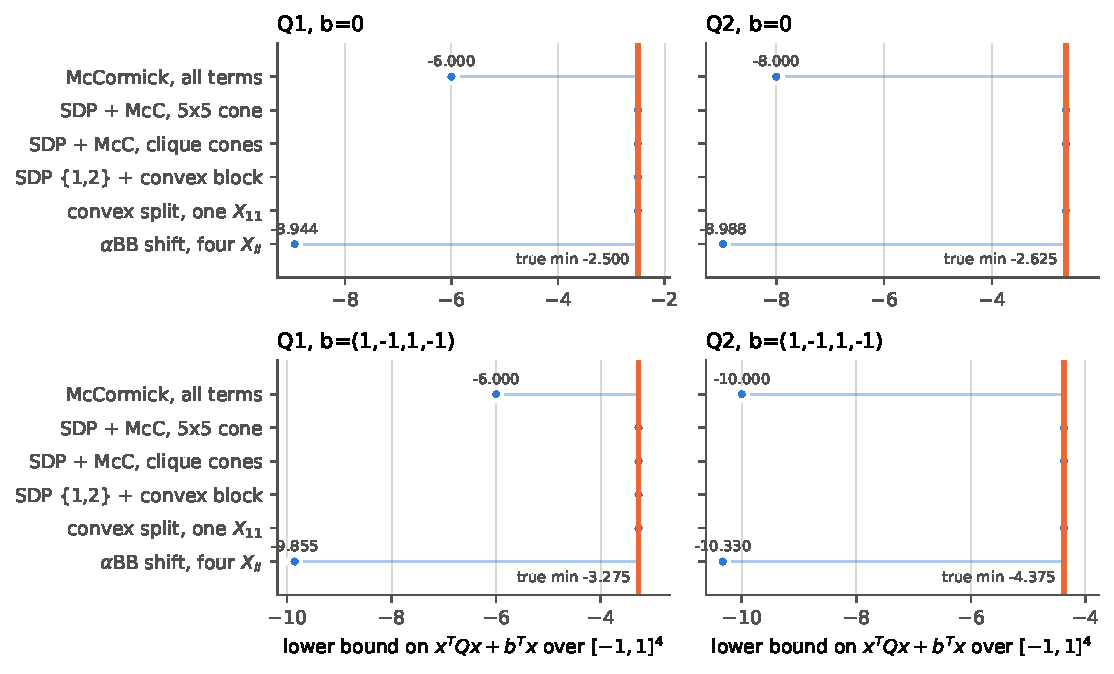
\includegraphics[width=0.95\textwidth]{figs/q1_bounds.pdf}
  \caption{Q1: lower bounds of six relaxations (dots) against the global minimum (vertical line).}
  \label{fig:q1}
\end{figure}

%======================================================================
\section*{Question 2: one bilinear term}

Write the constraint as $u\,v \le 2$ with
\[
  u = 1 - x_1 + 2x_2 - 2x_4 \in [-4, 6], \qquad v = 4x_2 - 5x_3 + x_4 + 2 \in [-8, 12].
\]
The bounds come from interval arithmetic and are attained at vertices of $[-1,1]^4$. With
$w \simeq uv$, the McCormick relaxation is
\begin{align*}
  w &\ge -8u - 4v - 32 \quad [(u+4)(v+8)\ge 0], &
  w &\le 12u - 4v + 48 \quad [(u+4)(12-v)\ge 0],\\
  w &\ge 12u + 6v - 72 \quad [(6-u)(12-v)\ge 0], &
  w &\le -8u + 6v + 48 \quad [(6-u)(v+8)\ge 0],
\end{align*}
and $w \le 2$. For a ``$\le$'' constraint only the two \emph{underestimators} matter. In the
original variables they read $8x_1 - 32x_2 + 20x_3 + 12x_4 \le 50$ and
$-12x_1 + 48x_2 - 30x_3 - 18x_4 \le 50$. The second normal is $-\tfrac32$ times the first, so
the whole relaxation is the slab
\[
  -\tfrac{100}{3} \;\le\; 8x_1 - 32x_2 + 20x_3 + 12x_4 \;\le\; 50 .
\]

\paragraph{Is lazy also good?}
The expanded product has \emph{eight} quadratic monomials. The usual alternative lifts each
one with its own McCormick inequalities. Sampling $10^6$ points of $[-1,1]^4$ gives:
\begin{itemize}
\item feasible: $53.7\%$;
\item single-term relaxation: $90.8\%$;
\item term-wise relaxation: $86.7\%$, contained in the single-term set on every sample.
\end{itemize}
Lower bounds for $u v$ over the box: true minimum $-18$, single-term LP $-48$, term-wise LP $-36$.
\begin{itemize}
\item The single term is much \emph{smaller}: one lifted variable and two cuts, against eight
  variables and $30$ inequalities.
\item It is also \emph{weaker}. The interval bounds treat $u$ and $v$ as independent, but they
  share $x_2$ and $x_4$, so the image of the box is the dashed polygon in
  Figure~\ref{fig:q2}(a). The McCormick corner $(u,v) = (6,-8)$, where $uv = -48$, cannot be
  reached.
\end{itemize}
Tighter bounds on $u, v$ do not help here, because each interval is exact on its own.

\begin{figure}[h]
  \centering
  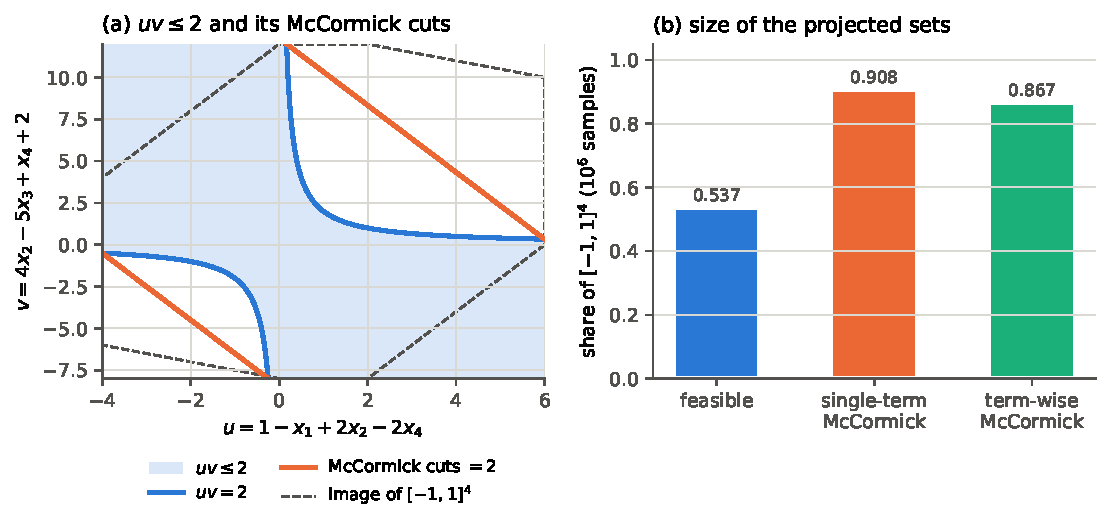
\includegraphics[width=0.95\textwidth]{figs/q2_mccormick.pdf}
  \caption{Q2: (a) the feasible set in $(u,v)$ and the two McCormick cuts; (b) share of the box kept
  by each relaxation.}
  \label{fig:q2}
\end{figure}

%======================================================================
\section*{Question 3: RLT for $f(x) = -x_1^2x_2^2 + 2x_1x_2^3 - x_2^4$}

\paragraph{Bounds and valid inequalities for the intermediate powers.}
On $[-1,1]^2$:
$X_{11}, X_{22} \in [0,1]$ and $X_{12}, X_{122}, X_{211} \in [-1,1]$.
Valid inequalities come from products of the bound factors $(1\pm x_1)$ and $(1\pm x_2)$:
\begin{itemize}
\item \emph{Degree 2} (10 products), for example:
  \begin{itemize}
  \item $X_{11} \le 1$, from $(1-x_1)(1+x_1)\ge0$;
  \item $X_{11} \ge \pm 2x_1 - 1$, from $(1\mp x_1)^2\ge0$;
  \item McCormick for $X_{12}$: $1 \pm x_1 \pm x_2 + X_{12} \ge 0$ and $1 \pm x_1 \mp x_2 - X_{12} \ge 0$.
  \end{itemize}
\item \emph{Degree 3} (20 products), for example:
  \begin{itemize}
  \item $(1-x_1)(1-x_2)^2 \ge 0$: \ $1 - x_1 - 2x_2 + 2X_{12} + X_{22} - X_{122} \ge 0$;
  \item $(1+x_1)(1-x_2^2) \ge 0$: \ $1 + x_1 - X_{22} - X_{122} \ge 0$.
  \end{itemize}
\item \emph{Degree 4} (35 products), including the sheet's example.
\end{itemize}

\emph{Caveat found by the LP:} the 65 bound-factor products alone imply only
$X_{11}, X_{22} \ge -\tfrac13$. The bounds $X_{11}, X_{22}, X_{1111}, X_{1122}, X_{2222} \ge 0$
(squares are nonnegative) have to be added explicitly.

\paragraph{The square.}
$f(x) = -\big(x_1x_2 - x_2^2\big)^2$, which is checked with sympy and in Lean.

\paragraph{The alternative relaxation (RLT-B).}
Set $w = x_1x_2 - x_2^2 \simeq X_{12} - X_{22}$. The exact range of $w$ on $[-1,1]^2$ is
$[-2, \tfrac14]$: the minimum is at $(-1,1)$, and the maximum $\tfrac14$ at $x_2 = x_1/2$
with $x_1 = \pm1$. Interval arithmetic gives only $[-2,1]$. Since $f = -w^2$ is concave in
$w$, its convex envelope on $[w_L,w_U]$ is the secant:
\begin{align*}
  \min\; t \quad\st\quad & t \ge -(w_L+w_U)\,w + w_Lw_U \;=\; \tfrac74 w - \tfrac12,
    \quad w = X_{12} - X_{22}, \quad w_L \le w \le w_U,\\
  & \text{McCormick inequalities for } X_{12}, \text{ tangents and secant for } X_{22}.
\end{align*}
RLT-B needs $4$ new variables and $10$ inequalities. RLT-A (all degree-$\le4$ products) needs
$12$ variables and $70$ inequalities.

\paragraph{Comparison} (Figure~\ref{fig:q3}).
\begin{itemize}
\item \emph{Root bound:} both give $-4 = \min f$, attained at $(-1,1)$.
\item \emph{Sub-boxes} ($4\times4$ partition of the box): RLT-A and RLT-B with exact $w$-bounds
  are exact on all 16. RLT-B with interval bounds on $w$ has gaps of up to $0.31$ in the
  corner boxes.
\item \emph{Pointwise underestimator} $\phi(x)$ = value of the relaxation with $x$ fixed:
  $\phi_A \ge \phi_B$ everywhere, and strictly so at $420$ of $441$ grid points. The mean gap
  $f - \phi$ is $2.23$ for RLT-A and $2.40$ for RLT-B.
\item \emph{Tilted objectives} $f + c\trps x$ ($12$ random $c$): both exact, because every
  minimiser is a box vertex, where RLT is exact.
\end{itemize}

\emph{Verdict.} RLT-A is the stronger relaxation: it dominates RLT-B pointwise. RLT-B gives
the same bounds on every box we tried at a fraction of the size, but \emph{only if} $w$ is
bounded well. With interval bounds it is visibly weaker. In a branch-and-bound code RLT-B
with bound tightening on $w$ is the better buy. Both can also be added together, since
both are valid.

\begin{figure}[h]
  \centering
  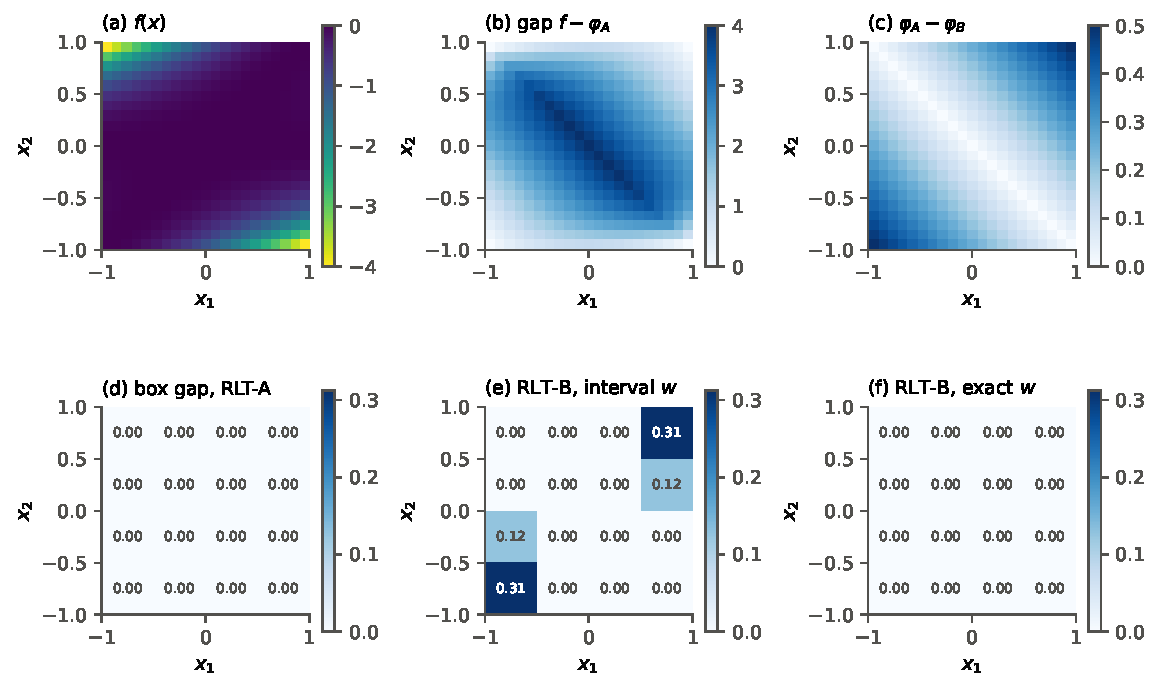
\includegraphics[width=0.95\textwidth]{figs/q3_quartic.pdf}
  \caption{Q3: (a) $f$; (b) gap of the RLT-A underestimator; (c) how much tighter RLT-A is than
  RLT-B; (d)--(f) lower-bound gaps on a $4\times4$ partition.}
  \label{fig:q3}
\end{figure}

%======================================================================
\section*{Question 4: $\min/\max\; x\trps Q x$ s.t.\ $x\trps x = 1$}

\paragraph{KKT conditions.}
With $\mathcal L = x\trps Qx - \mu\,(x\trps x - 1)$:
\[
  \nabla_x \mathcal L = 2Qx - 2\mu x = 0 \;\Longleftrightarrow\; Qx = \mu x, \qquad x\trps x = 1 .
\]
LICQ holds everywhere on the sphere because $\nabla(x\trps x) = 2x \ne 0$. So the KKT points are
exactly the unit eigenvectors, and the objective there is $x\trps Qx = \mu\, x\trps x = \mu$.

\paragraph{Why the minimum is the smallest eigenvalue.}
The sphere is compact, so a global minimiser exists. Since LICQ holds it is a KKT point, so
its value is the smallest KKT value, $\lambda_{\min}$. Moreover, the Hessian of the
Lagrangian on the tangent space $x^\perp$ is $2(Q - \lambda_k I)$, which is positive
semidefinite only for $\lambda_k = \lambda_{\min}$. So there are \emph{no} spurious local
minima. Equivalently, by the S-lemma the SDP relaxation
$\min\{\langle Q, X\rangle : \operatorname{tr} X = 1,\ X \succeq 0\}$ is exact.

\paragraph{Replacing $\min$ by $\max$} gives $\lambda_{\max}$, by the same argument applied to $-Q$.

\paragraph{The given $Q$.}
\begin{itemize}
\item Characteristic polynomial: $\det(Q - \mu I) = \mu^4 - 12\mu^3 + 42\mu^2 - 32\mu - 31$ (proved in Lean).
\item Eigenvalues: $\lambda = -0.534306,\ 2.322889,\ 4.061156,\ 6.150262$.
\item $\min = \lambda_{\min} \approx -0.5343$ at $x = \pm(-0.0598, -0.2711, -0.5847, 0.7622)$.
\item $\max = \lambda_{\max} \approx 6.1503$ at $x = \pm(-0.3261, 0.7013, -0.5909, -0.2295)$.
\end{itemize}
All 40 random Uno starts per problem converge to these values (Figure~\ref{fig:q4}), as the
missing spurious minima predict. Lean certifies the brackets
$\lambda_{\min} \in [-0.535, -0.534)$ and $\lambda_{\max} \in (6.150, 6.151]$, using rational
sum-of-squares certificates for $Q + 0.535I \succeq 0$ and $6.151I - Q \succeq 0$ and explicit
Rayleigh quotients.

\begin{figure}[h]
  \centering
  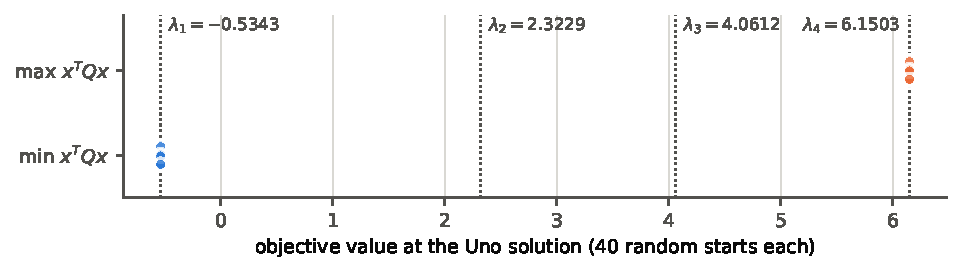
\includegraphics[width=0.85\textwidth]{figs/q4_eig.pdf}
  \caption{Q4: Uno solutions from 40 random starts each, against the spectrum of $Q$.}
  \label{fig:q4}
\end{figure}

%======================================================================
\section*{Verification, and do we need Lean?}

\paragraph{Proved in Lean 4 / Mathlib} (\code{lean/Globalopt/Basic.lean}, \code{lake build}, no \code{sorry}):
\begin{itemize}
\item \emph{Q1:}
  \begin{itemize}
  \item both convex splits;
  \item $d^* = 21/8$ is minimal;
  \item the global minima $\min x\trps Q_1x = -\tfrac52$ and $\min x\trps Q_2 x = -\tfrac{21}{8}$ on
    $[-1,1]^4$, both the bound and its attainment.
  \end{itemize}
\item \emph{Q2:} the interval bounds of $u, v$ and all four McCormick inequalities.
\item \emph{Q3:}
  \begin{itemize}
  \item $f = -(x_1x_2-x_2^2)^2$;
  \item the sheet's expansion of $(1-x_1)^2(1-x_2)^2$;
  \item the exact range $w \in [-2,\tfrac14]$;
  \item validity of the secant;
  \item $\min f = -4$.
  \end{itemize}
\item \emph{Q4:}
  \begin{itemize}
  \item at a KKT point the objective equals the multiplier, for any $n$;
  \item the characteristic polynomial;
  \item the eigenvalue brackets.
  \end{itemize}
\end{itemize}

\paragraph{Only checked numerically:}
\begin{itemize}
\item every LP/SDP bound and the comparisons between relaxations;
\item the chordal completion theorem, which is cited, not proved;
\item the claim that $\phi_A \ge \phi_B$, which was checked on a grid only.
\end{itemize}

\paragraph{Assessment.}
For identities and small polynomial inequalities, sympy and sampling already give high
confidence. Lean was not \emph{needed} for correctness, but it did add value:
\begin{itemize}
\item It turns ``the solver says $-2.625$'' into a proof of global optimality, using a
  certificate (sum of squares plus bound factors) that the agent had to find.
\item It forced exact rational data. For example, the eigenvalues can only be bracketed,
  never stated exactly.
\end{itemize}
The cost was a $\approx 8$\,GB Mathlib download and about $45$\,s of build time. The
\code{nlinarith} proofs went through once explicit product hints were supplied. Only the
$4\times4$ determinant needed a second attempt.

\paragraph{Reproduce.}
\begin{verbatim}
conda run -n optimization python q1_rlt.py  # and q2_mccormick.py,
                                            # q3_quartic.py, q4_eig.py
cd lean && lake build    # needs elan; first run: lake exe cache get
latexmk -pdf answers.tex
\end{verbatim}

\end{document}
